\chapter{Evaluation}
\label{ch:evaluation}

In diesem Kapitel werden die Ergebnisse der durchgeführten Experimente präsentiert, um die in Abschnitt \ref{sec:intro:goal} definierten Forschungsfragen zu beantworten.
Die Motivation für diese Untersuchung resultiert, wie bereits in der Einleitung dargelegt, aus den Erkenntnissen der Praxisphase bei der \ac{DFS}: Ein KI-gestützter Adjacent-Lotse muss nicht nur konfliktfrei, sondern auch effizient und für Menschen nachvollziehbar agieren. Ein zentrales Kriterium für diese \emph{Menschlichkeit} ist die Vermeidung unnötiger, kleinteiliger Kurskorrekturen ("Jittering"), die bei klassischen \ac{RL}-Ansätzen häufig auftreten.
\vspace{\baselineskip}

Um diesem Anspruch gerecht zu werden, wurde in Kapitel \ref{ch:konzeption} ein gemischter Aktionsraum konzipiert, der dem Agenten die explizite Entscheidungsmöglichkeit gibt, nicht einzugreifen (\emph{Noop}), aber dennoch die präzise Steuerung der Kursänderung mittes Gleitkommazahlen ermöglicht. Da Standard-Algorithmen wie PPO strukturelle Schwierigkeiten mit solchen Abhängigkeiten haben, wurde in Kapitel \ref{ch:ppo_bedingt} das \emph{Gradient Gating} als technische Lösung eingeführt.

Die Evaluation konzentriert sich daher auf zwei Hauptaspekte:
\begin{enumerate}
    \item \textbf{Technische Validierung:} Funktioniert der implementierte Gradient-Gating-Mechanismus wie beabsichtigt? Es muss nachgewiesen werden, dass die Anpassung des Algorithmus die fehlerhafte Gradientenberechnung für irrelevante Aktionen unterbindet, ohne die Lernstabilität in Standard-Problemen zu gefährden.
    \item \textbf{Operativer Vergleich:} Führt der Mehraufwand des gemischten Aktionsraums tatsächlich zu einem besseren Verhalten? Hierzu wird der neue Ansatz gegen einen klassischen Agenten mit rein diskreten Aktionen verglichen, insbesondere im Hinblick auf die Effizienz der Konfliktlösung und die Frequenz der Steuerbefehle.
\end{enumerate}

Dazu werden zunächst synthetische und standardisierte Tests durchgeführt, um die Korrektheit der Implementierung zu bestätigen. Anschließend erfolgt die Evaluation in der realistischen Flugverkehrssimulation.

\section{Methodik der Auswertung}
Die Bewertung erfolgt auf Basis der in Kapitel \ref{ch:Statistische_Auswertung} beschriebenen statistischen Methoden.
Da \ac{RL}-Training stochastischen Schwankungen unterliegt, reicht die Betrachtung einzelner Trainingsläufe nicht aus.
Als primäre Metrik zur Bewertung der Leistung wird daher der \emph{Interquartile Mean} (IQM) der episodischen Belohnungen (Rewards) verwendet. Dieser ist robuster gegenüber Ausreißern als der arithmetische Mittelwert. Ergänzend wird die \emph{Success Rate} (SR) als sekundäre Metrik herangezogen, um den operativen Erfolg (konfliktfreie Durchquerung des Sektors) zu quantifizieren.
Alle Metriken werden mit 95\%-Konfidenzintervallen mittels \emph{Percentile-Bootstrap} ausgewertet, um die statistische Signifikanz der Ergebnisse sicherzustellen und zufällige Effekte auszuschließen.

\section{Evaluation des Gradient-Gating-Mechanismus}
Bevor der Agent das komplexe Problem der Flugverkehrskontrolle angehen kann, muss die korrekte Funktionalität des implementierten Gradient-Gating-Mechanismus validiert werden. Dazu werden zwei Versuche durchgeführt:

\subsection{Versuch 1: Validierung der Funktionalität}
Um sicherzustellen, dass die Änderungen am PPO-Kern keine negativen Seiteneffekte auf die generelle Lernfähigkeit haben, wird der Mechanismus in einer bekannten Standard-Umgebung untersucht. Hierfür wird die OpenAI Gym Umgebung \texttt{LunarLanderContinuous-v3} gewählt.
In dieser Umgebung steuert der Agent ein Landefahrzeug, das sanft auf einer Plattform landen muss. 

\begin{figure}[h]
    \centering
    \includegraphics[width=0.6\textwidth]{chapters/bilder/lunar_lander.png}
    \caption{LunarLanderContinuous-v3}
    \label{fig:lunar_lander}
\end{figure}

Diese Umgebung wurde ausgewählt, da sie eine zum Flugverkehrskontrollproblem analoge Herausforderung bietet: Der Agent muss präzise kontinuierliche Aktionen wählen, um das Ziel zu erreichen. Das Standard-Szenario unterscheidet sich jedoch insofern, als dass Steuerbefehle teilweise in sogenannten Deadzones ignoriert werden, um die Statistische Warscheinlichkeit von Noop\hyp{}Aktionen im Trainingsprozess zu erhöhen.
\vspace{\baselineskip}

Deadzones sind konzeptionell problematisch, da sie Plateaus in der Belohnungslandschaft erzeugen.
In diesen Bereichen (siehe Abbildung \ref{fig:deadzone_plot}) ist der Gradient bezüglich der Aktion Null (\emph{Vanishing Gradient}), da Änderungen der Aktion keine Auswirkungen auf die Umgebung haben.
Der Algorithmus erhält somit kein Feedback, in welche Richtung die Policy verbessert werden muss, sodass der Agent nicht effektiv lernen kann, diese Bereiche zu verlassen oder gezielt zu nutzen. Eine detaillierte Beschreibung der Umgebung findet sich in der offiziellen Dokumentation \cite{lunar_lander_doc}.

\begin{figure}[htbp]
    \centering
    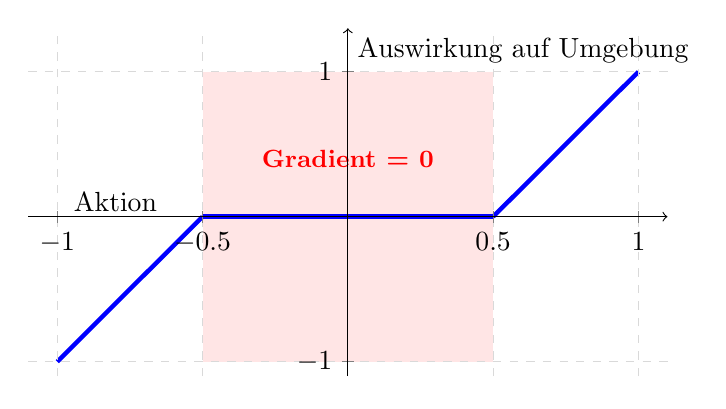
\begin{tikzpicture}
        \begin{axis}[
            width=0.8\textwidth,
            height=6cm,
            % xlabel is placed manually below using a node so it can be positioned
            % at a data coordinate (axis cs) in the negative region.
            ylabel={Auswirkung auf Umgebung},
            xmin=-1.1, xmax=1.1,
            ymin=-1.1, ymax=1.3,
            axis lines=middle,
            grid=major,
            grid style={dashed, gray!30},
            legend pos=north west,
            legend style={draw=none},
            xtick={-1, -0.5, 0, 0.5, 1},
            ytick={-1, 0, 1},
            % Improve axis line appearance
            axis line style={->},
            area style,
        ]
        
        % Deadzone shading
        \fill[red!10] (axis cs:-0.5,-1.0) rectangle (axis cs:0.5,1.0);
        
        % The function
        % Linear outside [-0.5, 0.5], zero inside
        \addplot[blue, ultra thick, domain=-1:-0.5] {2 * (x + 0.5)};
        \addplot[blue, ultra thick, domain=-0.5:0.5] {0};
        \addplot[blue, ultra thick, domain=0.5:1] {2 * (x - 0.5)};
        
        % Annotations
        \node[red, align=center, font=\small\bfseries] at (axis cs:0, 0.4) {Gradient = 0};

        % Manuelles xlabel an einer Datenkoordinate im negativen Bereich
        \node[align=center] at (axis cs:-0.8,0.1) {Aktion};

        \end{axis}
    \end{tikzpicture}
    \caption{Visualisierung des Deadzone-Problems: Die X-Achse repräsentiert die gewählte Aktion, die Y-Achse die resultierende Seitenschubdüsenleistung in der LunarLander-Umgebung.}
    \label{fig:deadzone_plot}
\end{figure}
\vspace{\baselineskip}

Die verwendeten Hyperparameter sind in Anhang \ref{lst:lunar_lander_hyperparams} dokumentiert. Der verwendete Environment Wrapper, der künstlich eine Abhängigkeit zwischen einer diskreten Aktivierungs-Aktion und der eigentlichen diskreten Steuerungsaktion erzeugt, ist in Listing \ref{lst:lunar_lander_wrapper} dargestellt. Dies ermöglicht den Vergleich der Lernkurven unter kontrollierten Bedingungen.
\vspace{\baselineskip}

Die zugrunde liegenden Hypothesen lauten wie folgt:
\begin{enumerate}
    \item \label{hyp:baseline} \textbf{Baseline-Performance:} Der Standard-PPO-Algorithmus erreicht in der regulären Umgebung eine durchschnittliche finale Belohnung von mindestens 270 \cite{algo_score_reference}.
    \item \label{hyp:no_gating} \textbf{Architektur-Robustheit:} Der PPO-Algorithmus ohne Gradient Gating zeigt in der modifizierten Umgebung keine signifikante Leistungsverschlechterung gegenüber dem Standard-PPO.
    \item \label{hyp:convergence} \textbf{Gating-Trade-off:} Der Einsatz von Gradient Gating führt initial zu einer verlangsamten Konvergenz (niedriger \emph{Mean Eval Mean}), resultiert jedoch in einer überlegenen finalen Policy (höherer \emph{Last Eval Mean}).
    \item \label{hyp:stability} \textbf{Stabilität:} Gradient Gating reduziert die Varianz zwischen den Trainingsläufen und erhöht die Lernstabilität signifikant.
    \item \label{hyp:Interferenzen} \textbf{Vermeidung negativer Interferenzen:} Die angepasste Netzarchitektur mit separaten Verarbeitungspfaden für diskrete und kontinuierliche Aktionen in Kombination mit Gradient Gating führt zu einer weiteren Leistungssteigerung gegenüber der Standard-Gradient-Gating-Variante, besonders in Scenarien mit eine hochen Anteil non -Noop Aktionen.
\end{enumerate}

\subsubsection*{Durchführung}

Um die Effektivität des Gradient-Gating-Mechanismus zu testen, werden vier Versionen des PPO-Algorithmus in dieser Umgebung trainiert:
\begin{enumerate}
    \item \textbf{Standard PPO:} Der unveränderte Basis-Algorithmus.
    \item \textbf{PPO mit Wrapper:} Eine mittels Wrapper modifizierte Umgebung, die den gemischten Aktionsraum simuliert.
    \item \textbf{PPO mit Wrapper und Gradient Gating:} Der Standard-Algorithmus in der modifizierten Umgebung, erweitert um den Gradient-Gating-Mechanismus.
    \item \textbf{PPO mit Gating und angepasster Architektur:} Zusätzlich zum Gradient Gating wird eine spezialisierte Netzarchitektur eingesetzt. Diese trennt die Verarbeitungspfade für diskrete und kontinuierliche Ausgaben, um negative Interferenzen zwischen den unterschiedlichen Lernzielen zu minimieren. Die Netzarchitektur sieht für jede Aktionskomponente separate Subnetzwerke vor. 
\end{enumerate}

Jede Konfiguration wird mit den selben Hyperparamertern und den gleichen 15 Seeds trainiert, um die Vergleichbarkeit der Ergebnisse zu gewährleisten. Beim Bootstrap wurden 5000 Stichproben gezogen. Die Trainingsdauer beträgt jeweils 3 Million Zeitschritte.


\subsubsection*{Ergebnisse}

\begin{table}[htbp]
    \centering
    \caption{Vergleich der Trainingsergebnisse (IQM mit 95\%-Konfidenzintervall)}
    \label{tab:evaluation_results}
    \begin{tabular}{l|ccc|ccc}
        \toprule
        & \multicolumn{3}{c}{\textbf{Last Eval Mean}} & \multicolumn{3}{c}{\textbf{Mean Eval Mean}} \\ 
        \textbf{Konfiguration} & \textbf{Low} & \textbf{IQM} & \textbf{High} & \textbf{Low} & \textbf{IQM} & \textbf{High} \\
        \midrule
        Standard PPO & 264.31 & 274.23 & 277.15 & 229.04 & 231.75 & 235.12 \\
        PPO (No Gating) & 266.87 & 275.03 & 279.86 & 224.91 & 229.86 & 235.33 \\
        PPO (Gating) & 282.46 & 283.50 & 284.54 & 130.73 & 157.66 & 177.86 \\
        PPO (Split Net) & 278.07 & 279.81 & 282.22 & 90.85 & 113.48 & 142.64 \\
        \midrule
        Paird (Gating - Standard) & 5.22 & 9.24 & 19.41 & -101.07 & -74.10 & -53.81 \\
        Paird (No Gating - Standard) & -9.17 & 0.96 & 12.51 & -7.61 & -2.03 & 4.38 \\
        Paird (Split Net - Standard) & 2.41 & 5.71 & 14.56 & -140.17 & -118.04 & -90.54 \\
        \bottomrule
    \end{tabular}
\end{table}

Die in Tabelle \ref{tab:evaluation_results} quantifizierten Daten ermöglichen eine detaillierte Überprüfung der aufgestellten Hypothesen.
Zunächst bestätigt sich die grundlegende Validität des Versuchsaufbaus: Der Standard-PPO erreicht mit einem IQM von 274.23 den geforderten Referenzwert (Hypothese \ref{hyp:baseline}). Wichtiger noch ist die Bestätigung von Hypothese \ref{hyp:no_gating}: Die Einführung der Wrapper-Struktur führt beim Basis-Algorithmus (`Paird No Gating - Standard`) zu keiner signifikanten Leistungsänderung, da das Konfidenzintervall $[-9.17, 12.51]$ die Null einschließt. Dies stellt sicher, dass alle im Folgenden beobachteten Effekte tatsächlich auf den Gating-Mechanismus und nicht auf die Umgebungskapselung zurückzuführen sind.

\subsubsection*{Der Trade-off zwischen Konvergenz und Endleistung}
Der Kern der Untersuchung, der postulierte "Trade-off" (Hypothese \ref{hyp:convergence}), tritt in den Ergebnissen deutlich hervor. Betrachtet man die durchschnittliche Leistung über das gesamte Training hinweg, ist der Standard-Algorithmus überlegen.

\begin{figure}[htbp]
    \centering
    \includegraphics[width=0.8\textwidth]{chapters/bilder/iqm_ci_LunarLanderContinuous-v3_mean_eval_mean.png}
    \caption{Durchschnittliche Trainingsleistung (IQM) über alle Episoden. Der niedrige Wert des Gating-Ansatzes (orange) visualisiert die anfänglichen Lernschwierigkeiten, durch die die hierarchische Struktur zunächst erlernt werden muss.}
    \label{fig:iqm_mean_eval}
\end{figure}

Wie in Abbildung \ref{fig:iqm_mean_eval} visualisiert, resultiert dies in einem signifikant niedrigeren \emph{Mean Eval Mean} für den Gating-Ansatz. Das strikt negative Paird-Intervall $[-101.07, -53.81]$ quantifiziert diesen Effekt und belegt die verlangsamte initiale Konvergenz. Der Agent muss zunächst lernen, die diskrete Entscheidung (Aktion oder Noop) korrekt zu treffen, bevor er die kontinuierliche Steuerung verfeinern kann.

Dieser initiale Investition zahlt sich jedoch am Ende des Trainings aus. Sobald die hierarchische Struktur erlernt ist, übertrifft der Gating-Mechanismus die Baseline deutlich. Das positive Paird-Intervall für die finale Leistung (`Last Eval Mean`: $[5.22, 19.41]$) bestätigt, dass das langsamere Lernen zu einer leistungsfähigeren finalen Policy führt.

\subsubsection*{Stabilität und Architektur-Entscheidungen}
Ein wesentlicher Vorteil des Gating-Ansatzes zeigt sich in der Robustheit der Ergebnisse (Hypothese \ref{hyp:stability}). Während die Standard-Varianten gegen Ende des Trainings eine höhere Varianz aufweisen, konvergiert der Gating-Ansatz sehr stabil.

\begin{figure}[htbp]
    \centering
    \includegraphics[width=0.8\textwidth]{chapters/bilder/iqm_ci_LunarLanderContinuous-v3_last_eval_mean.png}
    \caption{Finale Trainingsleistung (IQM) am Ende des Trainings. Der Gating-Ansatz zeigt nicht nur einen höheren Mittelwert, sondern durch das schmalere Intervall auch eine signifikant höhere Reproduzierbarkeit.}
    \label{fig:iqm_last_eval}
\end{figure}

Abbildung \ref{fig:iqm_last_eval} verdeutlicht dies durch die Spannweite der Konfidenzintervalle: Das Intervall der Gating-Variante ist mit einer Breite von 2.08 drastisch schmaler als das der Standard-Variante (12.84). Dies impliziert eine signifikant höhere Lernstabilität und Reproduzierbarkeit über verschiedene Random Seeds hinweg.

Überraschend sind hingegen die Ergebnisse bezüglich der Netzarchitektur (Hypothese \ref{hyp:Interferenzen}). Die spezialisierte \emph{Split Net}-Variante verbessert zwar die Leistung gegenüber der Baseline, bleibt jedoch mit einem IQM von 279.81 signifikant hinter der einfachen Gating-Variante (283.50) zurück. 
Dies widerlegt die Annahme, dass eine frühe Trennung der Netzpfade in diesem Szenario zwingend notwendig ist. Zwei Gründe scheinen hierfür ausschlaggebend: Erstens erhöht die spezialisierte Architektur die Komplexität des Modells, was sich in einer nochmals verlangsamten Konvergenz (Mean Eval IQM 113.48) niederschlägt. Zweitens ist der Anteil an Noop-Aktionen in der LunarLander-Umgebung im Vergleich zu Flugverkehrsszenarien relativ gering, wodurch negative Interferenzen weniger stark ins Gewicht fallen und die einfachere Architektur effizienter bleibt.

\subsubsection*{Analyse der Performance Profiles}
Einen tieferen Einblick in die Verteilung der Ergebnisse über alle Trainingsläufe hinweg bieten die Performance Profiles. Sie zeigen nicht nur Mittelwerte, sondern die Wahrscheinlichkeit, mit der ein bestimmtes Leistungsniveau erreicht wird.

\begin{figure}[htbp]
    \centering
    \includegraphics[width=0.8\textwidth]{chapters/bilder/perf_profile_LunarLanderContinuous-v3_last_eval_mean.png}
    \caption{Performance Profile der finalen Leistung (Last Eval). Die Gating-Variante (orange) zeigt stochastische Dominanz (Verlauf oben rechts), was bedeutet, dass sie über fast das gesamte Spektrum hinweg mit höherer Wahrscheinlichkeit bessere Ergebnisse liefert.}
    \label{fig:perf_profile_last_eval}
\end{figure}

In Abbildung \ref{fig:perf_profile_last_eval} ist die Überlegenheit des Gating-Ansatzes (orange Kurve) evident. Die Kurve verläuft stochastisch dominant gegenüber den Baselines, liegt also konstant weiter rechts oben. Besonders im Bereich sehr hoher Scores hält die Gating-Kurve ihr Niveau länger, was die zuvor diskutierte Robustheit visuell unterstreicht.

\begin{figure}[htbp]
    \centering
    \includegraphics[width=0.8\textwidth]{chapters/bilder/perf_profile_LunarLanderContinuous-v3_mean_eval_mean.png}
    \caption{Performance Profile der durchschnittlichen Leistung (Mean Eval). Hier fällt die Gating-Kurve früher ab, was die initialen "Kosten" des hierarchischen Lernprozesses grafisch darstellt.}
    \label{fig:perf_profile_mean_eval}
\end{figure}

Spiegelt man dies gegen die durchschnittliche Performance in Abbildung \ref{fig:perf_profile_mean_eval}, zeigt sich das exakte Gegenteil. Hier dominiert die Standard-PPO-Variante, während die Gating-Kurve deutlich früher abfällt. Dies ist die grafische Entsprechung des identifizierten Trade-offs: Der Preis für die überlegene Endleistung und Stabilität ist eine längere und "teurer" Trainingsphase zu Beginn.

\subsection{Versuch 2: Validierung in der Flugverkehrsumgebung}




\section{Evaluation des Aktionsraum-Designs}
\subsection{Vergleich: Gemischter vs. Diskreter Aktionsraum}
In diesem zentralen Experiment werden die Leistungsunterschiede zwischen dem neu konzipierten Agenten mit gemischtem Aktionsraum und einem Referenz-Agenten untersuchten. Der Referenz-Agent nutzt einen klassischen, rein diskreten Aktionsraum (feste Menge an Kursänderungen), wie er in vielen bisherigen Arbeiten verwendet wird.
Besonderes Augenmerk liegt hierbei nicht nur auf der reinen Konfliktfreiheit (Success Rate), sondern auf der Qualität der generierten Trajektorien: Wie oft greift der Agent ein? Wie effizient sind die Routen?

\section{Fazit der Ergebnisse}



